\documentclass[11pt,a4,oneside]{amsart}
\usepackage{geometry}                % See geometry.pdf to learn the layout options. There are lots.
%\geometry{a4paper}                   % ... or a4paper or a5paper or ... 
%\geometry{landscape}                % Activate for for rotated page geometry
\usepackage[parfill]{parskip}    % Activate to begin paragraphs with an empty line rather than an indent
\usepackage{xcolor}
\usepackage{graphicx}
\usepackage{amssymb}
\usepackage{epstopdf}
\usepackage{algorithm}
\usepackage{algorithmic}
\usepackage{subcaption}

\usepackage{sidecap}
\usepackage{hyperref}
\usepackage{xspace}
\usepackage{tcolorbox}
\DeclareGraphicsRule{.tif}{png}{.png}{`convert #1 `dirname #1`/`basename #1 .tif`.png}
\renewcommand{\baselinestretch}{1.2}

\usepackage{biblatex}
\addbibresource{references.bib}

%%%% Some handy commands
\newcommand{\Acc}{\mathcal A}
\newcommand{\Op}{\hat{\mathcal O}}
\newcommand{\bL}{\hat L}
\newcommand{\Cl}{Cl$^-$\xspace}
\newcommand{\HCO}{HCO$_3$\xspace}
\newcommand{\gabar}{GABA$_A$R\xspace}




%%%%%%%%%%%%%%%%%%%%%%%%%%%%%%%%%%%%%%%%%%%%%%%%%%%%%%%%%%%%%%%%%%%%%%
%%%%%%%%%%%%%%%%%%%%%%%%%%%%%%%%%%%%%%%%%%%%%%%%%%%%%%%%%%%%%%%%%%%%%%
\title[NE TNXXXX]{A universal model of consciousness \\  NE TNXXXX}
\author{R. Waters  and E. Gorov}
%\date{\today}           % Activate to display a given date or no date

%%%%%%%%%%%%%%%%%%%%%%%%%%%%%%%%%%%%%%%%%%%%%%%%%%%%%%%%%%%%%%%%%%%%%%
\begin{document}
\maketitle

\begin{abstract}
\normalsize
    In previous work,  Wendling et al. \cite{wendling02} demonstrated how NMMs can be used to generate realistic looking epileptic seizure transitions.  And so it goes.

\end{abstract}

%\clearpage
\tableofcontents


\clearpage
%%%%%%%%%%%%%%%%%%%%%%%%%%%%%%%%%%%%%%%%%%%%%%%%%%%%%%%%%%%%%%%%%%%%%%
\section{Introduction}
\label{sec:introduction}
The present document corresponds directly to \textbf{Task 1} in Galvani-lab TN002 (NE  TN0148), and summarizes our first attempt to generate both ictal and inter-ictal activity in a single NMM, using different modeling approaches, what we call the ``Patient Unified (SEEG) Network" model. With this simplified model, we aim to simulate the electrical activity in a node of the epileptogenic zone network (EZN), \textcolor{blue}{which can be connected to more NMM} in the future to simulate the propagation of epileptic activity to the irritable network (IN) and the propagation network (PN).

%%%%%%%%%%%%%%%%%%%%%%%%%%%%%%%%%%%%%%%%%%%%%%%%%%%%%%%%%%%%%%%%%%%%%%
\section{Spontaneous transitions: external input}
\label{sec:input}
In order to provide a physiologically realistic framework, we have  explored how to induce spontaneous transitions from inter-ictal state to seizure state based on variations of the external input received by the main pyramidal cell. The model is to be  ``autonomous" in the language of ODEs, with the sole exception of its dependence on inputs (from PNS or other CNS nodes). We may express this by
\begin{equation}
\dot u = f(u,p(t))
\label{eq:rate_equation}
\end{equation}
where $u$ represents the potential or its time derivative at different synapses. The only explicit time dependence allowed in the model is throught the external inputs, denoted by $p(t)$. 

Using Equation~\ref{eq:rate_equation}, we have explored the possibility of generating spontaneous transitions without changing the model parameters, but rather by stochastic changes of the external input received by the main pyramidal cell. This idea arises from the fact that a linear increase of the external input (with a superimposed white noise signal) leads to the transition from background activity to inter-ictal spikes and then to sustained spiking (ictal activity). This is illustrated by Figure~\ref{fig:linear}.

\begin{figure}[hbtp!]
    \centering
    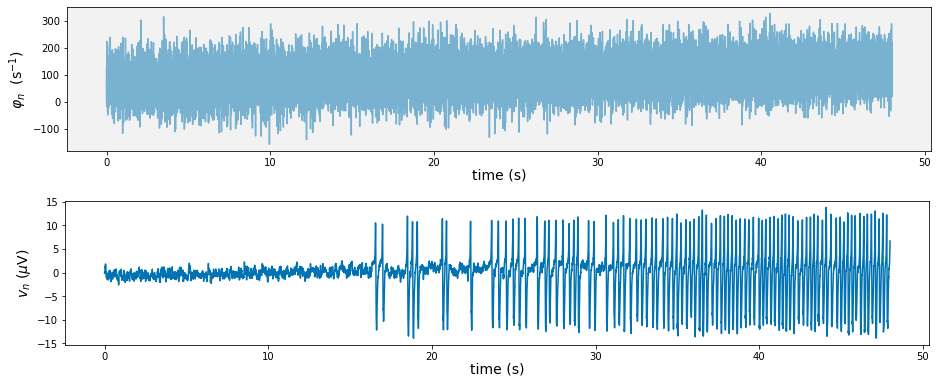
\includegraphics[width=15cm]{figures/Linear.png}
    \caption{{\bf A linear increase of the external input to the main pyramidal cell leads to inter-ictal spikes first and then to ictal activity with increasing frequency.} Top: The upper panel shows the external input, modelled as white noise with a mean value increasing from 70 to 130 s$^{-1}$, and standard deviation of 60 s$^{-1}$. Bottom:  membrane potential of main pyramidal.}
    \label{fig:linear}
\end{figure}


%%%%%%%%%%%%%%%%%%%%%%%%%%%%%%%%%%%%%%%%%%%
\bgroup
\def\arraystretch{1.2}
\begin{table}[hbtp!]
\centering
\caption{Parameters, description and standard values of the neural mass model.}
\label{table:params}
\footnotesize
\begin{tabular}{lll} 
\textbf{Parameter} & \textbf{Description} & \textbf{Value} \\ \hline
A & Average excitatory synaptic gain & 5 mV \\\hline
B & Average slow inhibitory synaptic gain & -42 mV \\\hline
G & Average fast inhibitory synaptic gain & -20 mV \\\hline
l/a & Time constant of average excitatory post synaptic potentials & a = 100 s$^{-1}$ \\\hline
l/b & Time constant of average slow inhibitory post synaptic potentials & b = 50 s$^{-1}$ \\\hline
1/g &Time constant of average fast inhibitory post synaptic potentials & g = 500 s$^{-1}$ \\\hline
C$_{pre \rightarrow post}$ & Average number of synaptic contacts between population types & \begin{tabular}[c]{@{}l@{}}C$_{E\rightarrow P}$ = 135\\ 
C$_{I_{slow}\rightarrow P}$ = 33.75 \\
C$_{I_{fast}\rightarrow P}$ = 108 \\
C$_{Ext\rightarrow P}$ = 1 \\
C$_{P\rightarrow E}$ = 135 \\
C$_{P\rightarrow I_{slow} }$ = 33.75 \\
C$_{P\rightarrow I_{fast}}$ = 40 \\
C$_{I_{slow}\rightarrow I_{fast} }$ = 13.5 \\
\end{tabular} \\\hline
$v_0, e_0, r$ & Parameters of the nonlinear asymmetric sigmoid function & \begin{tabular}[c]{@{}l@{}}v = 6 mV \\ e0 = 2.5 s$^{-1}$ \\ r = 0.56 mV$^{-1}$\end{tabular} 
 \\\hline
\end{tabular}
\end{table}
\egroup
%%%%%%%%%%%%%%%%%%%%%%%%%%%%%%%%%%%%%%%%%%%%%

\section{Conclusions}
We have used a ``Wendling class" neural mass model, which includes the following neuronal populations: a pyramidal cell, an excitatory interneuron, a fast inhibitory interneuron and a slow inhibitory interneuron. Realistic transitions from inter-ictal to ictal phase can be achieved in such a model by changing the synaptic gain of the different neuronal populations, in particular of the fast and slow inhibitory interneurons\footnote{Wendling, F., et al. ``Epileptic fast activity can be explained by a model of impaired GABAergic dendritic inhibition." European Journal of Neuroscience 15.9 (2002): 1499-1508.}. 

 
%%%%%%%%%%%%%%%%%%%%%%%%%%%%%%%%%%%%%%%%%%%%%%%%%%%%%%%%%%%%%%%%%%%%%%
\clearpage
  {\small
 \begin{tcolorbox}
 \section*{Annex: Further adventures of K}
{\Large K} couldn’t wait to begin her experiment. 
\ \\

Thanks to the NanoPatch technology just prototyped at Blazarlab, she would be the first person in history to monitor one million neurons at the same time. This would deliver a giant leap beyond Starstim-X. 
\ \\

NanoPatch promised to be a revolutionary development. Leveraging carbon nanotube growth control discoveries, the tool was able to follow the scent of chlorine in GABA receptors in dendrites to patch into multiple pyramidal cells at the same time. The output was massive data: up to several million streams carrying information about the cells' membrane potentials and firing rates.
\ \\

Furthermore, she could use the same nanotube channels to stimulate the cells. She could read and write into a cortical patch.
\ \\

Her in-vitro cortical patch, fresh from epilepsy surgery a few hours ago, was waiting. It was alive but resting, displaying some background activity, a faint buzz. She could almost feel it, and wondered “what is was like to be a severed cortical island”.
\ \\

The data stream was some large that she decided to collapse it to an average value for the entire set of neurons. This was a first test to validate so-called Neural Mass Models developed two centuries before. These mathematical models aimed to reproduce precisely this, the average behavior of a collective set of neurons.

The main point was, she knew Maxwell's equations. \ \\

\begin{equation}
\nabla \cdot E =\rho 
\end{equation}

 \end{tcolorbox} 
 }
 
\printbibliography

\end{document}  
